% !TEX program = xelatex
\documentclass[10pt,letterpaper,twocolumn]{article}

% === GEOMETRY ===
\usepackage[top=0.75in, bottom=0.75in, left=0.75in, right=0.75in]{geometry}

% === FONTS ===
\usepackage{fontspec}
\usepackage{unicode-math}

\setmainfont{Latin Modern Roman}
\setsansfont{Latin Modern Sans}

% Custom AC fonts
\newfontfamily\acbold{ywft-processing-bold}[
  Path=../../system/public/type/webfonts/,
  Extension=.ttf
]
\newfontfamily\aclight{ywft-processing-light}[
  Path=../../system/public/type/webfonts/,
  Extension=.ttf
]
\newfontfamily\kidlispfont{ComicRelief-Regular}[
  Path=fonts/,
  Extension=.ttf
]
\newfontfamily\kidlispbold{ComicRelief-Bold}[
  Path=fonts/,
  Extension=.ttf
]
\setmonofont{Latin Modern Mono}[Scale=0.85]

% === PACKAGES ===
\usepackage{xcolor}
\usepackage{titlesec}
\usepackage{enumitem}
\usepackage{booktabs}
\usepackage{tabularx}
\usepackage{multicol}
\usepackage{fancyhdr}
\usepackage{hyperref}
\usepackage{graphicx}
\graphicspath{{figures/}}
\usepackage{ragged2e}
\usepackage{microtype}
\usepackage{listings}
\usepackage{natbib}
\usepackage[colorspec=0.92]{draftwatermark}

% === COLORS (AC palette) ===
\definecolor{acpink}{RGB}{180,72,135}
\definecolor{acpurple}{RGB}{120,80,180}
\definecolor{acdark}{RGB}{64,56,74}
\definecolor{acgray}{RGB}{119,119,119}
\definecolor{klbrand}{RGB}{205,92,155}
\definecolor{klcyan}{RGB}{112,214,255}
\definecolor{kldark}{RGB}{48,43,58}
\definecolor{draftcolor}{RGB}{205,92,155}

% === DRAFT WATERMARK ===
\DraftwatermarkOptions{
  text=WORKING DRAFT,
  fontsize=3cm,
  color=draftcolor!18,
  angle=45,
  pos={0.5\paperwidth, 0.5\paperheight}
}

% === KIDLISP SYNTAX COLORS ===
\definecolor{klfn}{RGB}{0,136,170}
\definecolor{klform}{RGB}{119,51,170}
\definecolor{klrepeat}{RGB}{170,0,170}
\definecolor{klnum}{RGB}{204,0,102}
\definecolor{klstr}{RGB}{170,120,0}
\definecolor{klcmt}{RGB}{102,102,102}
\definecolor{klmath}{RGB}{0,136,0}
\definecolor{klvar}{RGB}{204,102,0}
\definecolor{klembed}{RGB}{0,136,0}

% KidLisp inline color macros
\newcommand{\kn}[1]{\textcolor{klnum}{#1}}
\newcommand{\kt}[1]{\textcolor{klstr}{#1}}
\newcommand{\kv}[1]{\textcolor{klvar}{#1}}
\newcommand{\ke}[1]{\textcolor{klembed}{\textbf{#1}}}
\newcommand{\km}[1]{\textcolor{klmath}{#1}}

% === HYPERREF ===
\hypersetup{
  colorlinks=true,
  linkcolor=acpurple,
  urlcolor=acpurple,
  citecolor=acpurple,
  pdfauthor={Jeffrey Alan Scudder},
  pdftitle={KidLisp '26: En minimal Lisp til generativ kunst},
}

% === SECTION FORMATTING ===
\titleformat{\section}
  {\normalfont\bfseries\normalsize\uppercase}
  {\thesection.}
  {0.5em}
  {}
\titlespacing{\section}{0pt}{1.2em}{0.3em}

\titleformat{\subsection}
  {\normalfont\bfseries\small}
  {\thesubsection}
  {0.5em}
  {}
\titlespacing{\subsection}{0pt}{0.8em}{0.2em}

% === HEADER/FOOTER ===
\pagestyle{fancy}
\fancyhf{}
\renewcommand{\headrulewidth}{0pt}
\fancyhead[C]{\footnotesize\color{acpink}\textit{Arbejdsudkast --- ikke til citation}}
\fancyfoot[C]{\footnotesize\thepage}

% === CUSTOM COMMANDS ===
\newcommand{\acdot}{{\color{acpink}.}}
\newcommand{\kidlisp}{\textsc{KidLisp}}

% === LISTINGS ===
\lstdefinelanguage{kidlisp}{
  morekeywords=[1]{wipe,ink,line,box,circle,tri,plot,flood,shape,zoom,scroll,spin,blur,contrast,embed,layer,width,height,frame,time,wiggle,melody,mic,suck,sort,form,trans,cube,move,scale,hop,overtone,resolution,write,text,type,stamp,paste,point,poly,noise,fade,pan,unpan,mask,unmask,flip},
  morekeywords=[2]{def,let,if,cond,once,later,lambda,do},
  morekeywords=[3]{repeat},
  morekeywords=[4]{random,sin,cos,tan,floor,ceil,round,abs,sqrt,min,max},
  sensitive=true,
  morecomment=[l]{;},
  morestring=[b]",
  escapeinside={|}{|},
}
\lstset{
  language=kidlisp,
  basicstyle=\ttfamily\small,
  keywordstyle=[1]\color{klfn}\bfseries,
  keywordstyle=[2]\color{klform}\bfseries,
  keywordstyle=[3]\color{klrepeat}\bfseries,
  keywordstyle=[4]\color{klmath},
  commentstyle=\color{klcmt}\itshape,
  stringstyle=\color{klstr},
  breaklines=true,
  frame=single,
  rulecolor=\color{acgray!30},
  backgroundcolor=\color{acgray!5},
  xleftmargin=0.5em,
  xrightmargin=0.5em,
  aboveskip=0.5em,
  belowskip=0.5em,
}

\lstdefinelanguage{json}{
  basicstyle=\ttfamily\small,
  stringstyle=\color{acpink},
  morestring=[b]",
  literate=
    {:}{{{\color{acgray}:}}}{1}
    {,}{{{\color{acgray},}}}{1}
    {\{}{{{\color{acgray}\{}}}{1}
    {\}}{{{\color{acgray}\}}}}{1},
}

% === LIST SETTINGS ===
\setlist[itemize]{nosep, leftmargin=1.2em, itemsep=0.1em}
\setlist[enumerate]{nosep, leftmargin=1.2em}

% === COLUMN SEPARATION ===
\setlength{\columnsep}{1.8em}

% === PARAGRAPH SETTINGS ===
\setlength{\parindent}{1em}
\setlength{\parskip}{0.3em}

\begin{document}

% ============ TITLE BLOCK ============

\twocolumn[{%
\begin{center}

\includegraphics[height=4em]{pals}\par\vspace{0.5em}
{\kidlispbold\fontsize{26pt}{30pt}\selectfont\color{kldark} Kid{\color{klbrand}Lisp} '26}\par
\vspace{0.2em}
{\kidlispfont\fontsize{11pt}{13pt}\selectfont\color{klbrand} En minimal Lisp til generativ kunst}\par
\vspace{0.6em}
{\normalsize Jeffrey Alan Scudder}\par
{\small\color{acgray} Aesthetic Inc.}\par
{\small\color{acgray} ORCID: \href{https://orcid.org/0009-0007-4460-4913}{0009-0007-4460-4913}}\par
\vspace{0.3em}
{\small\color{acpurple} \url{https://kidlisp.com} \enspace$\cdot$\enspace \url{https://aesthetic.computer}}\par
\vspace{0.6em}
\rule{\textwidth}{1.5pt}
\vspace{0.5em}
\end{center}

\begin{center}
{\small\color{acpink}\textbf{[ arbejdsudkast --- ikke til citation ]}}
\end{center}
\vspace{0.3em}

\begin{quote}
\small\noindent\textbf{Abstrakt.}
\kidlisp{} er en minimal Lisp-dialekt designet til generativ kunst og interaktive audiovisuelle oplevelser. Den kører inde i Aesthetic Computer, en browserbaseret kreativ computing-platform. Programmer gemmes i MongoDB, tildeles korte alfanumeriske koder og er eksekverbare via en URL. En 15.000-linjers træ-vandrende evaluator leverer 118 indbyggede funktioner, der spænder over tegning, farve, transformation, matematik, animation og lyd---uden fil-I/O, netværk eller generel strengmanipulation---hvilket gør det sikkert at eksekvere vilkårlig bruger-indsendt kode. Vi beskriver sprogdesignet, lagrings- og distributionsinfrastrukturen, mediepipelinen, og rapporterer om adoption af 59 forfattere, der har skabt over 16.000 programmer. Vi argumenterer for, at indlejring af social distribution direkte i et domænespecifikt sprog---frem for at bolte det på---producerer kvalitativt anderledes kreative kodningspraksisser.
\end{quote}
\vspace{0.5em}
}]

% ============ 1. INTRODUKTION ============

\section{Introduktion}

Kreative kodningsmiljøer kræver typisk, at brugere lærer et generelt programmeringssprog, før de producerer visuelt eller lydmæssigt output. Processing~\citep{reas2007processing} bruger Java; p5.js~\citep{mccarthy2015p5js} bruger JavaScript; Sonic Pi~\citep{aaron2016sonic} bruger Ruby-lignende konstruktioner. Selvom disse værktøjer dramatisk har sænket barrieren for computationel udtryk, kræver de stadig kendskab til variabler, funktioner, kontrolflow og---i mange tilfælde---et lokalt udviklingsmiljø.

\kidlisp{} udgår fra et andet spørgsmål: \emph{hvad er det mindste sprog, der kan producere interessant generativ kunst?} Svaret er en Lisp med omhyggeligt valgte indbyggede funktioner, ingen brugerdefinerede procedurer og en browser-native køretid, der ikke kræver installation. Et komplet animeret program kan være en enkelt linje:

\begin{lstlisting}
(ink |\kt{rainbow}|) (repeat |\kn{100}| |\kv{i}|
  (circle (wiggle width) (wiggle height) |\kn{10}|))
\end{lstlisting}

Designet er motiveret af observationer fra No Paint~(2020), et pixelkunst-værktøj, hvis fællesskab af ikke-tekniske brugere demonstrerede, at mennesker lærer computing gennem social deltagelse i software, de elsker. \kidlisp{} udvider denne indsigt til et programmeringssprog: hvert program er øjeblikkeligt delbart via en kort kode, synligt på en URL og indlejrbart i andre programmer.

Denne artikel beskriver sprogdesignet~(\S\ref{sec:design}), evaluatorarkitekturen~(\S\ref{sec:architecture}), lagrings- og distributionsinfrastrukturen~(\S\ref{sec:infrastructure}), mediepipelinen~(\S\ref{sec:media}) og adoptionsdata~(\S\ref{sec:evaluation}).

\begin{figure}[t]
\centering
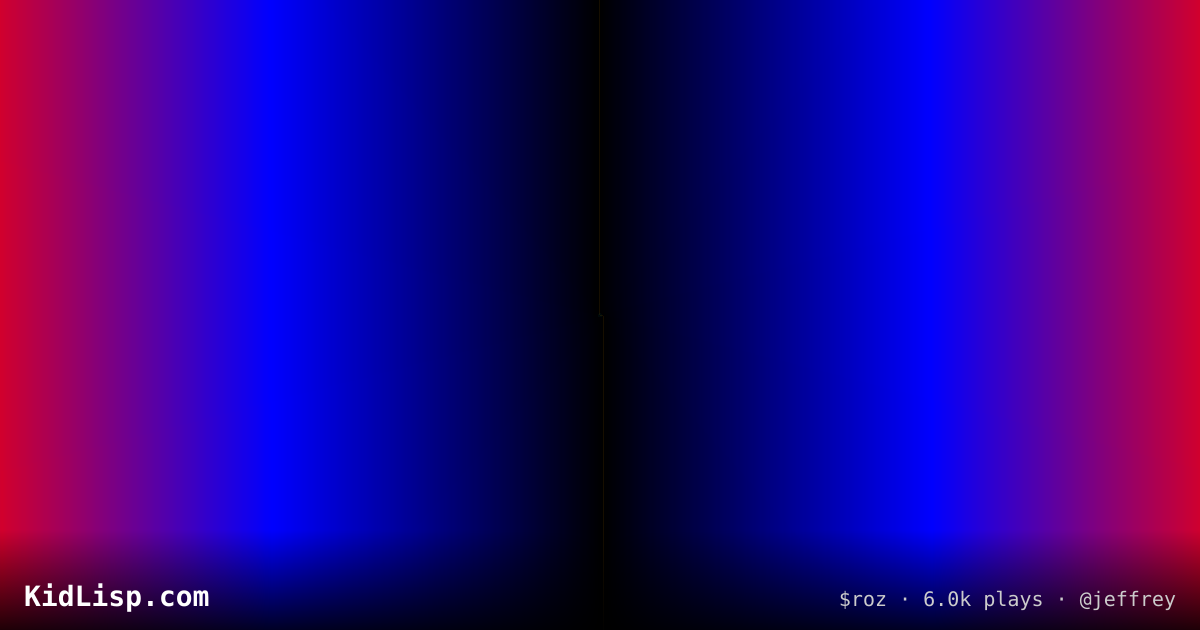
\includegraphics[width=\columnwidth]{kidlisp-og-mosaic.png}
\caption{Et fremhævet \kidlisp{}-program (\texttt{\$roz}) som renderet af oven-tjenesten til Open Graph sociale forhåndsvisninger. Overlejringen viser programkoden, afspilningstæller og forfatterhandle.}
\label{fig:og}
\end{figure}

% ============ 2. SPROGDESIGN ============

\section{Sprogdesign}
\label{sec:design}

\kidlisp{} er et S-udtrykssprog. Ethvert program er en sekvens af udtryk evalueret fra top til bund, der producerer sideeffekter på en HTML Canvas 2D-kontekst, en WebGL-kontekst, en Web Audio-graf eller en kombination heraf.

\subsection{Designprincipper}

\begin{enumerate}
  \item \textbf{Ethvert udtryk tegner.} Gyldig \kidlisp{} producerer synligt output. Der er intet \texttt{main}, ingen imports, intet boilerplate.
  \item \textbf{Fladt over dybt.} Programmer komponeres ved at indlejre andre programmer, ikke ved at definere abstraktioner. Dette holder koden læsbar ved et blik.
  \item \textbf{Sikkert ved konstruktion.} Ingen fil-I/O, intet netværk, ingen mutation af ekstern tilstand. Programmer er sandboxede af sprogets mangel på farlige primitiver.
  \item \textbf{Socialt som standard.} Hvert program får en kort kode og en URL. Deling er distributionsmekanismen, ikke en eftertanke.
\end{enumerate}

\subsection{Funktionskategorier}

De 118 indbyggede funktioner spænder over 12 kategorier (Tabel~\ref{tab:functions}).

\begin{table}[h]
\small
\centering
\begin{tabularx}{\columnwidth}{lrX}
\toprule
\textbf{Kategori} & \textbf{n} & \textbf{Eksempler} \\
\midrule
Grafik & 9 & \texttt{wipe}, \texttt{ink}, \texttt{line}, \texttt{box}, \texttt{circle} \\
Transformationer & 11 & \texttt{scroll}, \texttt{zoom}, \texttt{spin}, \texttt{blur}, \texttt{suck} \\
Matematik & 14 & \texttt{+}, \texttt{sin}, \texttt{cos}, \texttt{random}, \texttt{wiggle} \\
Farver & 19 & CSS-navne + \texttt{rainbow}, \texttt{zebra} \\
System & 9 & \texttt{width}, \texttt{height}, \texttt{frame}, \texttt{fps} \\
3D & 8 & \texttt{cube}, \texttt{form}, \texttt{trans}, \texttt{move} \\
Lyd & 6 & \texttt{mic}, \texttt{melody}, \texttt{overtone} \\
Kontrol & 7 & \texttt{def}, \texttt{if}, \texttt{repeat}, \texttt{once}, \texttt{later} \\
Tekst & 4 & \texttt{write}, \texttt{type}, \texttt{paste} \\
Input & 3 & \texttt{pen}, \texttt{touch} \\
Komposition & 4 & \texttt{embed}, \texttt{layer}, \texttt{fade} \\
Data & 4 & \texttt{let}, \texttt{list}, \texttt{get}, \texttt{set} \\
\midrule
\textbf{Total} & \textbf{118} & \\
\bottomrule
\end{tabularx}
\caption{Indbyggede funktioner efter kategori.}
\label{tab:functions}
\end{table}

\begin{figure}[t]
\centering
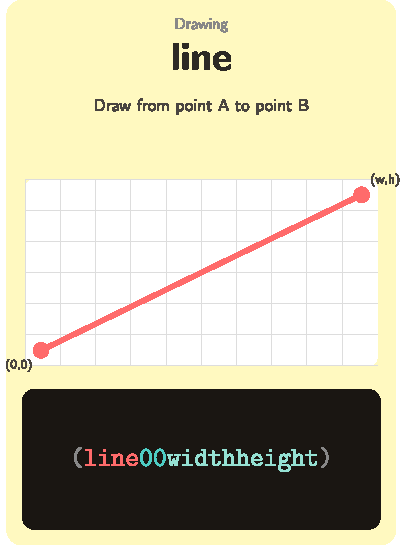
\includegraphics[height=4.5cm]{card-line.pdf}%
\hfill%
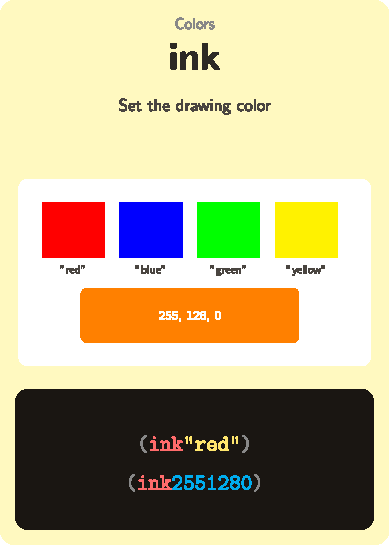
\includegraphics[height=4.5cm]{card-ink.pdf}
\caption{\kidlisp{} referencekort for funktionerne \texttt{line} og \texttt{ink}, der viser syntaks og koordinat-output. Kort distribueres som SVG-illustrationer på \texttt{kidlisp.com/cards}.}
\label{fig:cards}
\end{figure}

\subsection{Tidssyntaks}

\kidlisp{} leverer temporale operatorer, der planlægger udtryksevaluering uden eksplicitte løkker eller callbacks:

\begin{lstlisting}
|\kt{2.5s}| (wipe |\kt{red}|)           ; efter 2,5 sekunder
|\kt{1s...}| (spin |\kn{5}|)            ; gentag hvert sekund
|\kt{3s!}| (write "Done" |\kn{10}| |\kn{10}|)  ; affyr præcis én gang ved 3s
|\kt{30f}| (ink |\kt{blue}|)             ; efter 30 frames
\end{lstlisting}

Suffikset \texttt{s} betegner sekunder, \texttt{f} betegner frames, \texttt{...} betegner gentagelse, og \texttt{!} betegner engangseksekvering. Disse operatorer komponerer: \texttt{0.5s... (ink (random 255) (random 255) (random 255))} producerer en farveændring hvert halvt sekund.

\subsection{Hvad KidLisp udelader}

Sproget udelukker bevidst brugerdefinerede funktioner (ud over \texttt{def} til navngivne værdier), rekursion, strengmanipulation, fil-I/O, netværk, mutable datastrukturer og undtagelseshåndtering. Disse udeladelser \emph{er} designet. Ved at fjerne abstraktionsmekanismer forbliver programmer flade og læselige---en læser kan forstå ethvert program fra top til bund uden at spore kaldstakke.

% ============ 3. ARKITEKTUR ============

\section{Evaluatorarkitektur}
\label{sec:architecture}

Evaluatoren (\texttt{kidlisp.mjs}, 15.161 linjer) er et enkelt JavaScript ES-modul, der implementerer en træ-vandrende fortolker.

\subsection{Evalueringsmodel}

Evaluatoren kører én gang per animationsframe. S-udtryk tokeniseres og parses til et indlejret array-AST, derefter vandres med dispatch på det første symbol i hver liste. Indbyggede funktioner afbildes direkte til Canvas 2D-operationer, WebGL-kommandoer, Web Audio API-kald og matematiske beregninger. Hele programmet re-evalueres hvert frame, med \texttt{frame}- og \texttt{time}-bindinger opdateret automatisk---en immediate-mode model, der eliminerer eksplicitte animationsløkker.

\subsection{Deterministisk rendering}

Givet det samme tilfældige frø og frame-tal producerer et program altid identisk output. \texttt{random}-funktionen bruger en seedet PRNG initialiseret fra programmets korte kode, hvilket muliggør reproducerbar generativ kunst.

\subsection{Kaostilstand}

Ugyldig eller tilfældig tekstinput udløser kunstnerisk visuelt output frem for fejlmeddelelser. En konfidens-scoret detektor undersøger ordgenkendelsesrate ($<$30\% kendte ord), special-tegnforhold ($>$50\%) og parentesbalance (forhold $>$3:1) for at klassificere input som kode eller kaos. Kaotisk input producerer deterministisk generative visuals seedet fra inputteksten. Det betyder, at \emph{enhver} tekst skrevet i \kidlisp{} producerer noget visuelt---der er ingen fejltilstande synlige for brugeren.

\subsection{Ydeevne}

Evaluatoren implementerer tre optimerignsniveauer:

\begin{itemize}
  \item \textbf{Flerniveau-kodecache}: Indlejret programopløsning tjekker RAM, derefter IndexedDB, derefter netværk, derefter TEIA (et decentraliseret arkiv). Cache-hits undgår genparse og genhentning.
  \item \textbf{Buffer-pooling}: Op til 8 genbrugelige offscreen-canvases per opløsning, hvilket undgår allokeringschurn under kompositing.
  \item \textbf{Auto-densitet-skalering}: Pixeltæthed justeres mellem 0,5x og 4x baseret på et rullende FPS-gennemsnit (mål: 30--55 FPS), med 60-frame afkøling mellem justeringer.
\end{itemize}

Funktionskaldresultater, alfa-justerede pixelbuffere og blandingskompositorer caches individuelt og ugyldiggøres per frame.

% ============ 4. INFRASTRUKTUR ============

\section{Lagring og distribution}
\label{sec:infrastructure}

\subsection{MongoDB-lagring}

Hvert program gemmes som et dokument i \texttt{kidlisp} MongoDB-samlingen:

\begin{lstlisting}[language=json]
{
  "code": "cow",
  "source": "(wipe blue)\n(ink yellow)...",
  "hash": "a3f2e8...",
  "when": "2025-06-15T...",
  "lastAccessed": "2026-03-01T...",
  "hits": 342,
  "user": "auth0|abc123"
}
\end{lstlisting}

\texttt{hash}-feltet (SHA-256 af den trimmede kildekode) håndhæver indholdsadresseret deduplikering: identiske programmer opløses altid til den samme kode. \texttt{hits}-tælleren og \texttt{lastAccessed}-tidsstemplet muliggør brugsanalyser. Samlingen vedligeholder unikke indekser på både \texttt{code} og \texttt{hash}, plus sparse-indekser på \texttt{user} og valgfrie NFT-prægeregistreringer (\texttt{kept.network}).

\subsection{Kodegenerering}

Korte koder genereres af en kildebevidst algoritme. Systemet forsøger først at udlede en meningsfuld kode fra programmets indhold---ekstraktion af dominerende funktionsnavne, farvenøgleord eller strukturelle mønstre---med fallback til tilfældig \texttt{nanoid}-generering, hvis alle udledte koder er optaget. Dette producerer koder som \texttt{cow} (et program med ko-lignende former) frem for vilkårlige alfanumeriske strenge.

\subsection{REST API}

Lagringsendepunktet (\texttt{store-kidlisp.mjs}) leverer fem forespørgselstilstande over en enkelt URL:

\begin{enumerate}
  \item \textbf{POST} --- Gem et program. Deduplikerer via SHA-256-hash, genererer en kort kode, synkroniserer valgfrit til ATProto (Bluesky) og publicerer en profilhændelse.
  \item \textbf{GET \texttt{?code=xyz}} --- Hent et enkelt program med forfatterens handle opløst via \texttt{\$lookup} på \texttt{@handles}-samlingen.
  \item \textbf{GET \texttt{?codes=a,b,c}} --- Batchhentning (op til 50 koder) til indlejret lagopløsning under evaluering.
  \item \textbf{GET \texttt{?recent=true}} --- Pagineret feed sorteret efter oprettelsestid eller hit-antal, med valgfrit \texttt{handle}-filter til per-bruger-feeds.
  \item \textbf{GET \texttt{?stats=functions}} --- Funktionsbrugsanalyser på tværs af korpusset, returnerer vægtede tællinger efter programpopularitet.
\end{enumerate}

Autentificering er valgfri med en 3-sekunders timeout---anonym programoprettelse understøttes, men autentificerede brugere får tilskrivning og profilhændelsespublicering.

\subsection{Indlejring og komposition}

\texttt{\$code}-syntaksen inde i et program udløser en hentning fra lagrings-API'en (eller cache-hit), evaluering i en offscreen-buffer og kompositing på forældrens lærred. Dette skaber en rettet acyklisk kompositionsgraf. Et reelt eksempel:

\begin{lstlisting}
; Et 3D-gitter af kuber med indlejrede lag
(wipe |\kt{black}|)
(def |\kv{gridsize}| |\kn{6}|)
(repeat (|\km{*}| |\kv{gridsize}| |\kv{gridsize}|) |\kv{i}|
  (ink (hop |\kn{0.1}| |\kt{rainbow}| |\kt{blue}| |\kt{white}|))
  (form (trans (cube |\kv{i}|)
    (move (|\km{*}| (|\km{\%}| |\kv{i}| |\kv{gridsize}|) |\kn{3}|) |\kn{0}| |\kn{-20}|)
    (scale |\kn{1.5}|) (spin |\kn{0}| |\kn{1}| |\kn{0}|))))
(|\ke{\$27z}|)
(|\ke{\$cow}|)
\end{lstlisting}

Her opløses \texttt{\$27z} og \texttt{\$cow} fra MongoDB, renderes til offscreen-buffere og kompositeres. Brugere bygger komplekse visuals ved at lagre simple programmer frem for at skrive komplekse enkeltprogrammer.

% ============ 5. MEDIEPIPELINE ============

\section{Mediepipeline}
\label{sec:media}

Oven-tjenesten (\texttt{oven.aesthetic.computer}) konverterer optagne \kidlisp{}-sessioner til delbare medieaktiver.

\subsection{Optagelse til MP4}

Når en bruger optager en session, uploader sessionsserveren en ZIP med PNG-frames og valgfri WAV-lyd. Ovenen:

\begin{enumerate}
  \item Udpakker frames og læser \texttt{timing.json} for per-frame varigheder
  \item Genererer en thumbnail fra det midterste frame (3x nærmeste-nabo opskalering, tilpasset til 512$\times$512)
  \item Koder til H.264/AAC MP4 via FFmpeg med nærmeste-nabo opskalering for at bevare pixelkunst-æstetik
  \item Uploader til DigitalOcean Spaces CDN
  \item Gemmer bake-metadata i \texttt{oven-bakes} MongoDB-samlingen og underretter abonnenter via WebSocket
\end{enumerate}

Ovenen overvåger \texttt{tapes} MongoDB-samlingen via en ændringsstrøm og detekterer automatisk nye optagelser, der kræver behandling.

\begin{figure}[t]
\centering
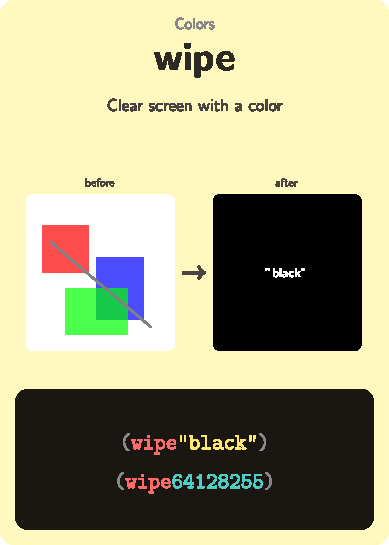
\includegraphics[height=4.5cm]{card-wipe.pdf}%
\hfill%
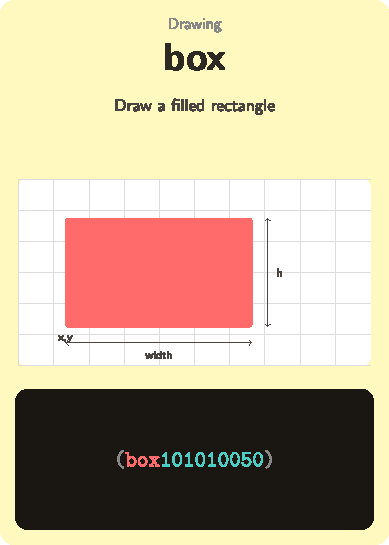
\includegraphics[height=4.5cm]{card-box.pdf}
\caption{Referencekort for \texttt{wipe} (ryd skærm med farve) og \texttt{box} (tegn rektangel). Hvert kort viser funktionssignaturen, et visuelt eksempel på et gitter og den tilhørende kildekode.}
\label{fig:cards2}
\end{figure}

\subsection{Sociale forhåndsvisningsbilleder}

Ovenen genererer Open Graph forhåndsvisningsbilleder til social deling på stabile URL'er (f.eks. \texttt{/kidlisp-og.png}). iOS-crawlere kræver direkte billedservering---de vil ikke følge 301-omdirigeringer på \texttt{og:image}-URL'er---så ovenen cacher genererede PNG'er og serverer dem med øjeblikkelige 200-svar, mens den udløser asynkron regenerering ved cache-miss.

\subsection{Aktivlevering}

Alle medieaktiver serveres via DigitalOcean Spaces CDN (\texttt{art-aesthetic-computer.sfo3.cdn.\allowbreak digitaloceanspaces.com}). Optagne bånd bruger en separat bucket (\texttt{at-blobs-aesthetic-computer}) med et valgfrit tilpasset CDN-domæne. Netlify proxyer \texttt{/preview/*} og \texttt{/icon/*} stier til ovenen for transparent URL-opløsning.

% ============ 6. IDE ============

\section{Udviklingsmiljø}

\kidlisp{} IDE'et på \texttt{kidlisp.com} leverer en Monaco-baseret editor med tilpasset syntaksfremhævning, et live forhåndsvisnings-iframe, der kører Aesthetic Computer-køretiden, et konsolpanel og afspilningskontroller (play/pause/stop).

En ``slide-tilstand'' tillader trækning af numeriske literaler i editoren for at justere værdier i realtid---markøren bliver en horisontal skyder over ethvert tal, og forhåndsvisningen opdateres kontinuerligt under trækningen.

IDE'et understøtter to layout-tilstande: \emph{studio} (delt-rude editor, forhåndsvisning og konsol) og \emph{scene} (editor overlejret direkte på fuldskærmslærredet med gennemsigtig baggrund, al krom skjult). Scenetilstand er designet til live performance-kontekster, hvor koden selv bliver del af det visuelle output.

% ============ 7. UDVIKLINGSHISTORIE ============

\section{Udviklingshistorie}
\label{sec:history}

Den følgende tidslinje er rekonstrueret fra git-historikken for Aesthetic Computer-repositoriet (626 commits, der berører \texttt{kidlisp.mjs} mellem april 2024 og marts 2026).

\subsection{Fase 1: Prototype (april--juni 2024)}

Udviklingen begyndte 17. april 2024 med en commit med titlen ``mock lisp.'' Inden for tre dage fungerede S-udtryksparser, \texttt{ink} og \texttt{line} accepterede numeriske parametre, og programmer kunne indtastes direkte i AC-prompten. I slutningen af april blev \texttt{def} tilføjet til variabeldefinitioner. Maj og juni 2024 oplevede 66 commits med tilføjelse af kernetegnefunktioner, \texttt{later}-tidskonstruktionen, \texttt{once} til engangseksekvering og anonym publicering af programmer. Evaluatoren nåede ca. 1.000 linjer.

\subsection{Fase 2: Pause (juli 2024--maj 2025)}

Ingen commits berørte \texttt{kidlisp.mjs} i 11 måneder. Sproget eksisterede som en fungerende prototype indlejret i AC-prompten, men manglede en lagringsbackend, indlejring, lyd eller en dedikeret editor.

\subsection{Fase 3: Hurtig udvidelse (juni--august 2025)}

Udviklingen genoptoges i juni 2025 med 82 commits den måned. Evaluatoren voksede fra 1.760 til 4.965 linjer i august. Nøgletilføjelser:

\begin{itemize}
  \item \textbf{Juni 2025}: Melodiparser, ursyntaks, per-frame renderingsmodel, testsuite (\texttt{kidlisp-spec.js}).
  \item \textbf{Juli 2025}: MongoDB-lagringsbackend (\texttt{store-kidlisp.mjs}), kort kode-generering, QR-kodedeling, båndoptagelse og GIF-eksport, mikrofoninput (\texttt{mic}) med fallback-animationer.
  \item \textbf{August 2025}: Indlejrede lag (\texttt{\$code}-syntaks) med alfakompositing og offscreen-buffering, Tezos-blockchain-integration til prægning af programmer som NFT'er, \texttt{fade}-gradienter og pixelbufferoptimeringer.
\end{itemize}

Evaluatoren krydsede 10.000 linjer i slutningen af september 2025.

\subsection{Fase 4: Platformintegration (september--december 2025)}

Med 108 commits alene i oktober (den travleste måned) integrerede denne fase \kidlisp{} i det bredere Aesthetic Computer-økosystem:

\begin{itemize}
  \item \textbf{September 2025}: Lag 0-arkitektur (slettetilstand), bake-lagdeling til MP4-eksport, ydeevnekritiske indlejrede lagrettelser.
  \item \textbf{Oktober 2025}: ATProto/Bluesky-føderation (programmer syndikeret som sociale medieopslag), PACK-tilstand til platformuafhængig bundling, slide-tilstand til realtids numerisk parameterjustering.
  \item \textbf{November 2025}: \texttt{kidlisp.com} IDE lanceret (Monaco-editor, live forhåndsvisning, konsol, afspilningskontroller), eksekverings-tracesystem til debugging, NFT-workflow omdøbt fra ``OBJKT'' til ``keep.''
  \item \textbf{December 2025}: Referencekort (SVG-illustrationer for hver funktion), IPFS-thumbnailgenerering til NFT'er, oven OG-billedgenerering til social deling, auto-densitet ydeevneskalering.
\end{itemize}

\subsection{Fase 5: Forfining (januar--marts 2026)}

Evaluatoren stabiliserede sig på 15.161 linjer. Tilføjelser inkluderede kaostilstand (februar 2026), 3D-primitiver (\texttt{cube}, \texttt{form}, \texttt{trans}), frekvensbånd lydvariabler, \texttt{flip}-kommandoen og scenetilstand til live performance. Udviklingen skiftede fra funktilføjelse til robusthed: rettelse af indlejrede lag-ydeevneregressioner, forebyggelse af kaostilstandsfejlklassificering og forbedring af cache-ugyldiggørelse.

\begin{table}[h]
\small
\centering
\begin{tabular}{lrl}
\toprule
\textbf{Dato} & \textbf{Linjer} & \textbf{Milepæl} \\
\midrule
Apr 2024 & 0 & Første commit (``mock lisp'') \\
Jun 2024 & $\sim$1{,}000 & Kernetegning, timing, variabler \\
Jun 2025 & 1{,}760 & Udvikling genoptages \\
Aug 2025 & 4{,}965 & Indlejring, lyd, lagring \\
Sep 2025 & 10{,}382 & Lagarkitektur, bagning \\
Dec 2025 & 13{,}877 & IDE, kort, OG-billeder \\
Feb 2026 & 15{,}161 & Kaostilstand, 3D, forfining \\
\bottomrule
\end{tabular}
\caption{Evaluatorvækst efter linjetælling (\texttt{kidlisp.mjs}).}
\label{tab:growth}
\end{table}

% ============ 8. EVALUERING ============

\section{Evaluering}
\label{sec:evaluation}

Adoptionsmetrikker per marts 2026 er vist i Tabel~\ref{tab:adoption}.

\begin{table}[h]
\small
\centering
\begin{tabular}{lr}
\toprule
\textbf{Metrik} & \textbf{Værdi} \\
\midrule
Totale programmer oprettet & 16.174 \\
Unikke forfattere & 59 \\
Programmer per forfatter (median) & 12 \\
Programmer per forfatter (øverste kvartil) & 180+ \\
Indlejringsdybde (maks. observeret) & 7 lag \\
Platform-registrerede brugere & 2.798 \\
\bottomrule
\end{tabular}
\caption{Adoptionsmetrikker (marts 2026).}
\label{tab:adoption}
\end{table}

\subsection{Funktionsbrugsanalyser}

\texttt{?stats=functions} API-endepunktet leverer vægtede funktionsbrugstællinger på tværs af korpusset. Det scanner op til 5.000 programmer (sorteret efter hits), parser hver kildekode for at udtrække funktionskald og returnerer tællinger vægtet efter programpopularitet. Dette muliggør kvantitativ analyse af, hvilke primitiver brugerne graviterer mod. De mest brugte funktioner er \texttt{wipe}, \texttt{ink}, \texttt{repeat} og \texttt{circle}---hvilket bekræfter, at brugere primært engagerer sig med tegning og iteration.

\subsection{Observationer}

\textbf{Komposition over abstraktion.} Brugere indlejrer snarere end abstraherer. De mest refererede programmer er simple visuelle primitiver (gradienter, former, mønstre), der fungerer som byggeklodser.

\textbf{Udforskning over ingeniørkunst.} Programmer er typisk korte (under 10 linjer). Brugere itererer ved at gemme nye programmer frem for at redigere eksisterende, hvilket skaber divergerende udforskningsstier synlige i lagringstidsstempler.

\textbf{Social læring.} De mest produktive forfattere begyndte med at se og remixe eksisterende programmer. Kort kode-systemet gør opdagelse tilfældig---brugere møder programmer ved at prøve tilfældige koder.

\subsection{Begrænsninger}

\kidlisp{} er ikke egnet til generel programmering, komplekse simulationer eller applikationer, der kræver tilstandsvedvarenhed på tværs af sessioner. Manglen på brugerdefinerede funktioner begrænser programkompleksitet---et bevidst valg, men ét som nogle avancerede brugere finder frustrerende.

% ============ 8. RELATERET ARBEJDE ============

\section{Relateret arbejde}

\textbf{Kreativ kodning.} Processing~\citep{reas2007processing} og p5.js~\citep{mccarthy2015p5js} er de dominerende værktøjer. OpenFrameworks bruger C++. Alle kræver håndtering af en projektstruktur og forståelse af et generelt programmeringssprog.

\textbf{Live-kodning.} Hydra~\citep{hydra2019} leverer browserbaseret live visuel kodning med JavaScript-metodekædekobling, men ingen persistent lagring eller sociale funktioner. Sonic Pi~\citep{aaron2016sonic} målretter musikuddannelse. Fluxus~\citep{fluxus2007} brugte Scheme til 3D-visuals, men vedligeholdes ikke længere.

\textbf{Uddannelsessprog.} Scratch~\citep{resnick2009scratch} demonstrerede, at social deling driver engagement i uddannelsesmæssig programmering. \kidlisp{} arver denne indsigt, men bruger tekstbaseret Lisp-syntaks og målretter generativ kunst snarere end generel uddannelse.

\textbf{Lisp til kunst.} Rackets \texttt{2htdp/image}-bibliotek~\citep{racket2018} leverer funktionel billedkonstruktion til CS-uddannelse, men målretter statiske billeder og pædagogik, ikke realtidsanimation med social distribution.

% ============ 9. KONKLUSION ============

\section{Konklusion}

\kidlisp{} demonstrerer, at et minimalt domænespecifikt sprog---browser-native, ingen brugerdefinerede abstraktioner, understøttet af en indholdsadresseret database med social distribution---kan understøtte et produktivt fællesskab af generative kunstpraktikere. Den centrale designindsigt er, at social distribution (korte koder, URL-deling, indlejring) ikke er en tilføjelse, men en kernesprogfunktion, der former, hvordan brugere lærer, skaber og bygger videre på hinandens arbejde.

Indlejringsgrafen, funktionsbrugsanalyse-API'en og korpusset af 16.000+ tidsstemplede programmer med forfattertilskrivning udgør et datasæt til studiet af kreative kodningspraksisser, computationel kreativitet og hvordan ikke-ekspertbrugere lærer funktionel programmering gennem social deltagelse.

\kidlisp{} er open source under ISC-licensen. Evaluatoren, dokumentation og værktøjer er tilgængelige på \url{https://github.com/digitpain/aesthetic.computer}. Programmer kan gennemses og oprettes på \url{https://kidlisp.com}.

\vspace{0.5em}
\noindent\textbf{ORCID:} \href{https://orcid.org/0009-0007-4460-4913}{0009-0007-4460-4913}

\vspace{0.5em}\noindent\textit{Oversat fra engelsk. Originalversion tilgængelig på \url{https://papers.aesthetic.computer}}

% ============ REFERENCES ============

\bibliographystyle{plainnat}
\bibliography{references}

\end{document}
